\documentclass{article}
\usepackage{pdfpages}
\begin{document}
	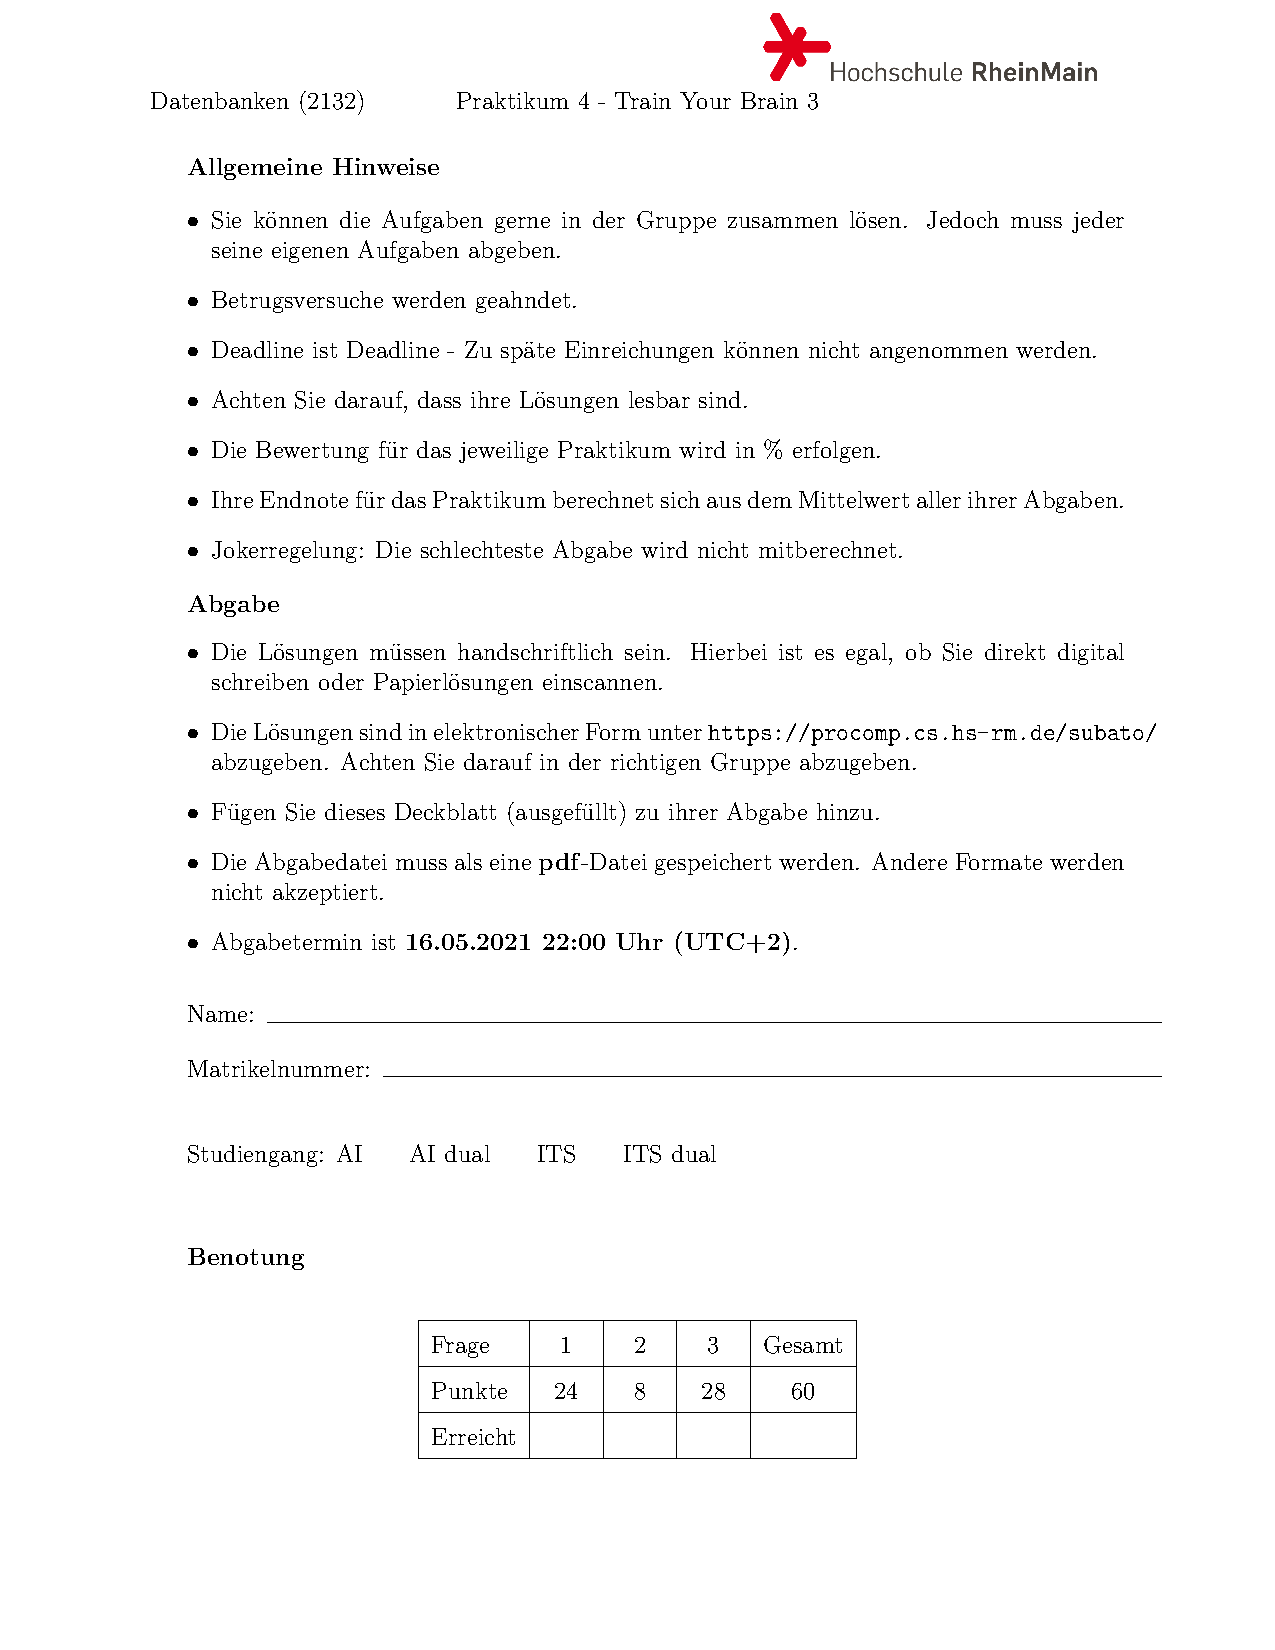
\includepdf[pages=1]{PA4_v2}
	\section*{Lsg Vorschlag DBÜ04 Maximilian Maag}
	AIdual, 1246281, Maag
	\begin{tabular}{c|c|c}
		a & b & c \\
		\hline
		\hline
		
	\end{tabular}
	\subsection*{Aufgabe 1}
	\subsection*{a)}
	R = 
	\begin{tabular}{c|c|c}
	a & b & c \\
	\hline
	\hline
	3 & 5 & 7 \\
	3 & 5 & 7 \\
	\end{tabular}
	\subsection*{b)}
	S = 
	\begin{tabular}{c|c|c}
		a & b & c \\
		\hline
		\hline
		5 & 7 & 9 \\
	\end{tabular}
	\subsection*{c)}
	S = 
	\begin{tabular}{c|c|c}
		a & b & c \\
		\hline
		\hline
		8 & 8 & 9 \\
		1 & 2 & 3
		
	\end{tabular}
	\subsection*{d)}
	S = 
	\begin{tabular}{c|c|c}
		a & b & c \\
		\hline
		\hline
		1 & 2 & 3
	\end{tabular}
	\subsection*{e)}
	SUM(R.a) = 7
	\subsection*{f)}
	AVG(R.b) = 4
	\subsection*{g)}
	8
	\subsection*{h)}
	3
	\subsection*{i)}
	$\rho$ = 
	\begin{tabular}{c|c}
		a & b\\
		\hline
		\hline
		1 & 3 \\
		2 & 10
	\end{tabular}
	\subsection*{j)}
	\begin{tabular}{c|c}
		a & b \\
		\hline
		\hline
		 1&2 \\
		 3&5 \\
		 3&5
	\end{tabular}
	\subsection*{k)}
	$\rho$ = 
		\begin{tabular}{c|c|c}
		d & c & x \\
		\hline
		\hline
		9 & 8 & 8 \\
		9 & 7 & 5 \\
		3 & 2 & 1
	\end{tabular}
	\subsection*{l)}
	$\rho$ = 
	\begin{tabular}{c|c}
		b & c \\
		\hline
		\hline
		2 & 3 \\
		5 & 7 \\
		5 & 7
	\end{tabular}
	\subsection*{Aufgabe 2}
	\subsection*{a)}
	$\pi_{alle Atrribute von R}(R \bowtie S)$
	\subsection*{b)}
	$\pi_{alle Atrribute von S}(R \bowtie S)$
	\subsection*{c)}
	S - $\pi_{alle Atrribute von S}(R \bowtie S)$
	\subsection*{d)}
	R - $\pi_{alle Atrribute von R}(R \bowtie S)$
	\subsection*{Aufgabe 3}
	\subsection*{a)}
	A := Drachen $\bowtie_{Drachen.art=did} Drachenkunde$
	\subsection*{b)}
	A := Drachen B := Drachen \\
	$\pi$(A $\bowtie$ B)
	\subsection*{c)}
	A := Drachen B := Drachen \\
	$\pi_{A.did, B.did}$ (A $\bowtie$ B)
	\subsection*{d)}
	A := $\delta_{art = "Flugdrache"}(Drachenkunde)$ \\
	B := A $\bowtie_{did=Drachen.art}$ Drachen \\
	C := B $\bowtie$ Aufenthalt \\
	D := $\pi_{fid}(C)$ \\
	$\pi_{fid,name,Stadt} (D \bowtie Farm)$
	\subsection*{e)}
	A := $\delta_{jahr > 2017 AND Gewicht \geq 1000}(Entwicklung)$ \\
	A := A $\bowtie$ Aufenthalt \\
	C := $\pi_{did,besitzer}(B \bowtie Farm)$ \\
	D := C $\bowtie$ Drachen  \\
	E := D $\bowtie$ Drachen \\
	$\pi_{besitzer, did, Drachenkunde.art, beschreibung}(E)$
	\subsection*{f)}
	$\gamma_{Jahr, min(laenge) \to laenge}(Entwicklung)$
	\subsection*{g)}
	A := $\gamma_{Jahr, min(laenge) \to laenge}(Entwicklung)$ \\
	B := A $\bowtie$ Entwicklungg \\
	C := B $\bowtie$ Drachen \\
	$\pi_{did,name,jahr,laenge}(C)$
	\subsection*{h}
	A := $\gamma_{did, max(ejahr) \to ejahr}(Aufenthalt)$ \\
	B := A $\bowtie$ Aufenthalt \\
	$\pi_{did, fid}(B)$
\end{document}